\subsection{Deploying Science Pipelines Releases}
\label{sec:scipipe-deploy}

DM has 3 primary types of ``release'', each with a different cadence, for
science pipeline related products.

\begin{enumerate}
    \item \texttt{daily} (also referred to as a \texttt{nightly})
    \item \texttt{weekly}
    \item \texttt{cycle} or ``major'' release, which have historically occurred
        once per DM planning cycle\ref{sec:agile}.
\end{enumerate}

A ``major'' release includes a human edited ``changelog'', updated installation
instructions, usage notes, a formal data processing characterization report,
etc\.  and thus can not be completely machine automated.  However, the
mechanical steps of tagging, building, and publishing software does share
jenkins pipeline code with the automatically triggered \texttt{daily} and
\texttt{weekly} releases.

The cadences of the \texttt{daily} and \texttt{weekly} releases are self
explanatory and are fully automated. They are triggered by jenkins on a fixed
schedule.

\subsubsection{Overview of ``Weekly Release'' pipeline}
\label{sec:releases_weekly}
\label{sec:releases_daily}

The ``weekly'' and ``nightly'' release pipelines are highly similar and
principally differ in that a ``nightly'' release does not tag \texttt{git}
repositories.  The rationale being that a ``nightly'' is used both for
developer convenience and as a ``canary'' to ensure that code changes have not
broken the release workflow but they are not a product that needs to be
reproducible/rebuildable from source, infinitely far into the future.  Both
release types share a library of common jenkins pipeline methods and are
planned to be merged in the near future into a single pipeline script that uses
only separate external configuration per release type.

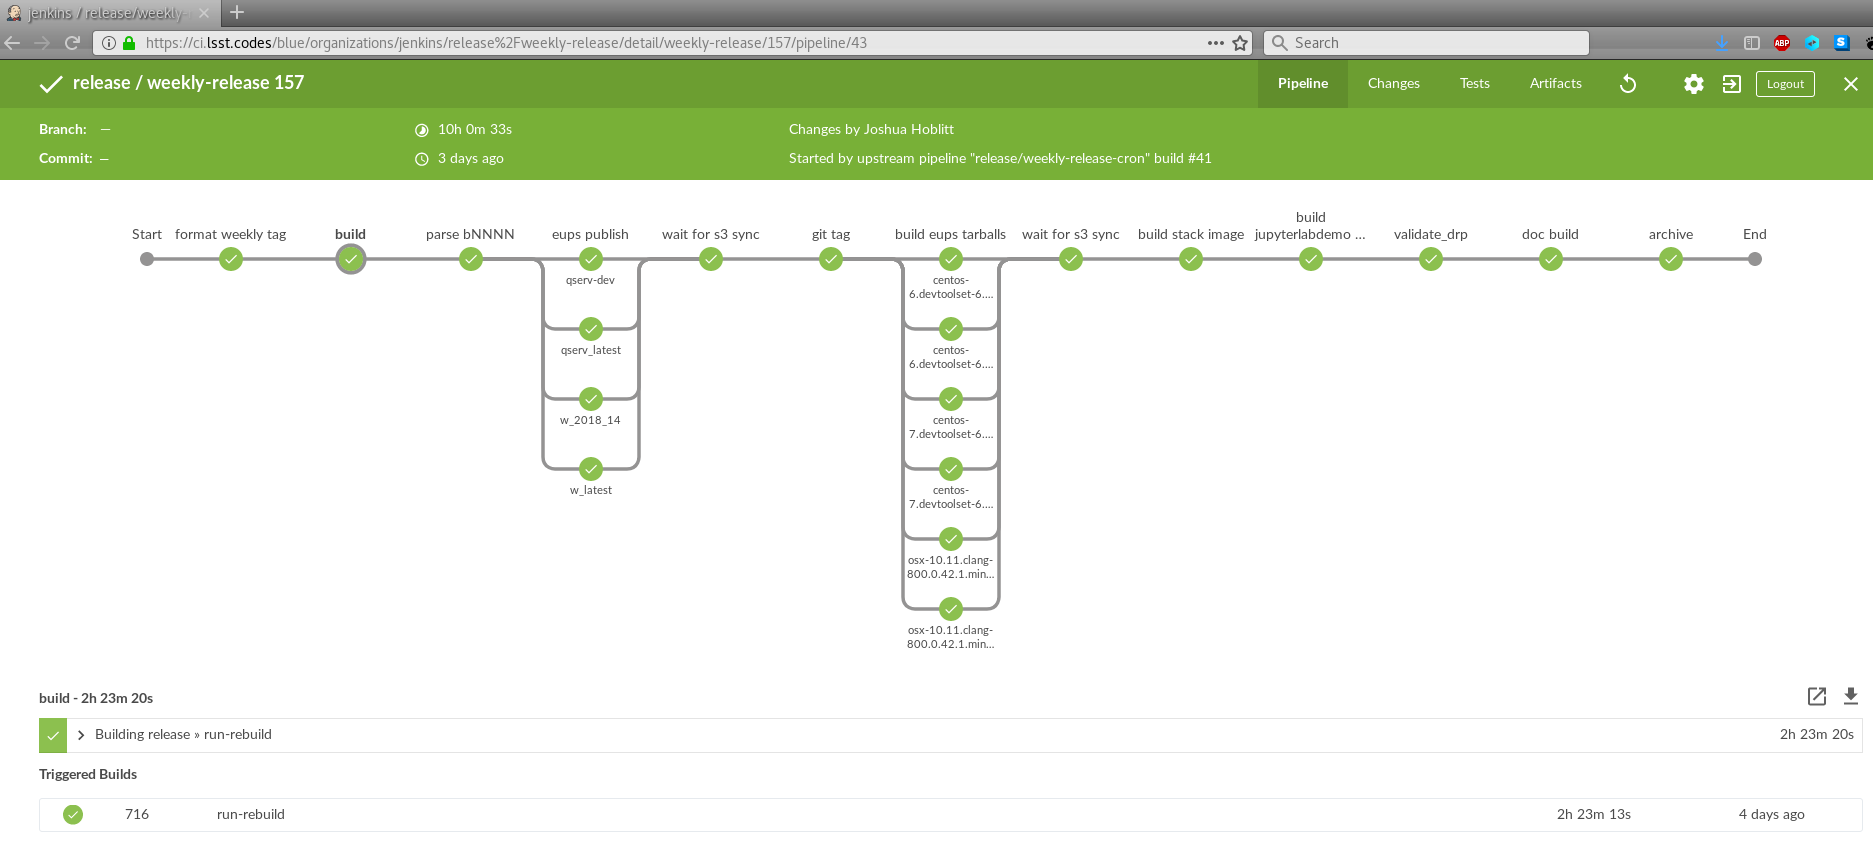
\includegraphics[width=0.7\textwidth]{pipelinedeploy-weekly-release}

\paragraph{``touchstone'' build + publish doxygen docs}

The first step in producing a release is to make a build from the
\texttt{master} branch of the source git repositories on the ``reference''
platform, which is presently \texttt{centos 7}.  If the per product unit tests
and a ``quick'' integration test succeed, a cross-package \texttt{HTML}
formatted documentation set is built using \texttt{doxygen} and is published to
a service that developers may access with a web-browser.

A ``manifest'' listing the \texttt{eups} products that were part of the build,
git repo sha1s for those products, and build dependencies is recorded by
\texttt{lsst\_build} at this stage in a git repo structure which the tool
refers to as ``versiondb''.  The canonical ``versiondb'' instance for science
pipeline releases is published on github as
\texttt{lsst/versiondb}FOOTNOTE:URL-https://github.com/lsst/versiondb.

\paragraph{publish eups source packages}
\label{sec:scipipe-deploy}

\texttt{eups}\ref{sec:eups} ``source packages'' or \texttt{eupspkg} are
produced from the installation tree resulting from the prior step.  Note that
although \texttt{eupspkg} are source based, and do not contain binary objects,
they require a complete binary installation as input to the packaging process.
In addition the \texttt{eupspkg}, a \texttt{eups} ``distrib tag'' is also
published, which is used to refer to a specific set of packages at fixed
versions.  Examples of \texttt{eups} tags: \texttt{w\_2018\_14}, \texttt{d\_2018\_04\_10}.

The \texttt{eupspkg} are pushed to an AWS S3 ``bucket'', which is used as the
canonical repository for both source and binary \texttt{eups} packages.  The S3
bucket is not publicly accessible as \texttt{eups} only supports remote
package repositories over \texttt{http[s]} that have \texttt{HTML} ``index
pages'' in the traditional format produced by the \texttt{apache}
webserverFOOTNOTE:URL-https://httpd.apache.org/.  To accommodate this
requirement, the S3 bucket is periodically replicated to a simple
serviceFOOTNOTE:URL-https://github.com/lsst-sqre/deploy-eups-pkgroot that
deploys on kubernetesFOOTNOTE:URL-https://kubernetes.io/ cluster which consists
of \texttt{TLS} termination, a reverse proxied apache instance, a persistent
storage volume, and a replication script.  The publicly accessible URL for
source packages is presently \url{https://eups.lsst.codes/stack/src/}.

\paragraph{tag git repos}

A script contained in
\texttt{sqre-codekit}FOOTNOTE:URL-https://github.com/lsst-sqre/sqre-codekit
uses the initial build ``manifest'' to apply an annotated git tag to all
repositories from which an \texttt{eups} product was pulled as part of the
build along with a number of ancillary git repositories that contain build
scripts, documentation, etc\. that would be needed to exactly reproduce the
release.

\paragraph{build/publish eups binary ``tarball'' packages}

This is perhaps the most complex stage in a release.  Multiple builds+publishes
are run in parallel.  As of the \texttt{15.0} (\texttt{eups} distrib tag
\texttt{v15\_0}) release, the build matrix is:

\begin{center}
    \begin{tabular}{| l | l |}
        \hline
        platform & python version \\ \hline
        centos-6 & py2 \\ \hline
        centos-6 & py3 \\ \hline
        centos-7 & py2 \\ \hline
        centos-7 & py3 \\ \hline
        osx-10.9 & py2 \\ \hline
        osx-10.9 & py3 \\
        \hline
    \end{tabular}
\end{center}

Every build is started from scratch and bootstraps a development/installation environment using the \texttt{newinstall.sh}FOOTNOTE:URL-https://github.com/lsst/lsst/blob/master/scripts/newinstall.sh script, just as an ``end user'' would when building/installing science pipeline software. Eg.

\begin{verbatim}
curl -sSL https://github.com/lsst/lsst/blob/master/scripts/newinstall.sh | bash -s -- -cb
\end{verbatim}

Then a \texttt{eups distrib install} is performed, also as an end-user would
run.  This is followed by publishing \texttt{eups} ``distrib tarballs'' (binary
package) to a local path.  \texttt{newinstall.sh} is again installed but into a
new path.  The second, pristine, installation pointed at the local publication
path, rather than the public \texttt{EUPS\_PKGROOT} and does a complete binary
installation.  This is followed by some simple acceptance tests, such as
building another package from source against the binary installation.  If there
are no failures, the binary ``tarballs'' are then publicly published in a
similar manner to the ``source'' \texttt{eupspkg} but using a different
directory prefix to prevent source and binary packages from different
environments from being intermixed.

\paragraph{build docker image}

A docker imageFOOTNOTE:URL-https://github.com/lsst-sqre/docker-tarballs is
constructed with the ``tarballs'' from the release pre-installed, which is
published to docker hub in the
\texttt{lsstsqre/centos}FOOTNOTE:URL-https://hub.docker.com/r/lsstsqre/centos/
repo.

The \texttt{sconsUtils}FOOTNOTE:URL-https://github.com/lsst/sconsUtils based
build/installation that is used by all science pipelines software, installs
virtually all files from the build tree. This includes \texttt{.o} files, unit
test scripts, test data, and \texttt{doxygen} \texttt{.html} output. In
addition, none of the executable binaries have been \texttt{strip(1)}d.  These
excess materials, that are unlikely to be of interest to a end user or in a
production system, would add approximate 6 GiB to uncompressed docker image and
would result an overall size around 10 GiB.  To avoid frustrating downstream
consumers, the aforementioned items are stripped from the docker layer.

\paragraph{build jupyterlab docker image}

The ``release'' docker image is used as the base (\texttt{FROM}) for the
jupterlabdemo base image.  This, theoretically, results in there being both
``nightly'' and ``weekly'' builds becoming available in a jupyterlab environment
with relatively low latency.

\paragraph{process test data sets and collect metrics}

The ``release'' docker image is also used to run several test data sets using a
package called
\texttt{validate\_drp}FOOTNOTE:URL-https://github.com/lsst/validate\_drp/.
Metrics are collected from the processing results and are shipped to a
dashboard called ``SQuaSH''FOOTNOTE:URL-https://squash.lsst.codes/, which plots
trends over time.

\paragraph{experimental doc build+publish}

Due to the ease of ``composition'' with jenkins pipeline, it is relatively low
cost to additional pipeline stages on a temporary basis in order to test out
new features.  Presently, this stage is ``tacked on'' to the regular release
workflow in order to evaluate a new documentation build+publish in parallel
with the existing \texttt{doxygen} based build.
